\documentclass{standalone}
\usepackage{tikz}
\usetikzlibrary{shapes, arrows, positioning}
\begin{document}
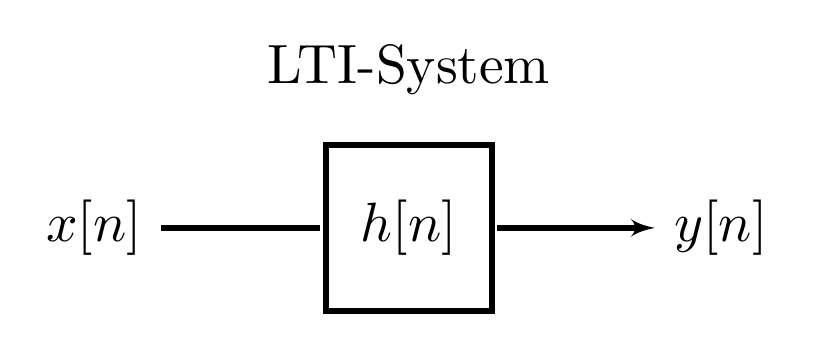
\begin{tikzpicture}[auto,>=latex', transform shape, scale=2]

\tikzstyle{block} = [draw, shape=rectangle, minimum height=3em, minimum width=3em, node distance=2cm, line width=2pt]

%Creating Blocks and Connection Nodes
\node at (0,0) (input) {$x[n]$};
\node [block, right of=input] (h) {$h[n]$};
\node [above of = h]{LTI-System};
\node [right = of h] (output) {$y[n]$};

%Conecting Blocks
\draw[->, line width=2pt] (input) -- (h) -- (output);

\end{tikzpicture}
\end{document}
